%!TEX root = thesis.tex

\chapter{Motion planning}
\label{chap:moveit}
This chapter explains the motion planning related part of the thesis. The introduction gives an overview about motion planning problems in general. Further on, the sampling based motion planning approach is described. Subsequent sections describe the integration of the motion planning framework \emph{MoveIt} into the existing robot setup.

\section{Introduction}

\citep[p. 1--11]{choset2005} describes motion planning as to be the task of finding a collision free path from one robot \emph{configuration} to another one. The classic path planning problem is the so called \emph{piano mover's problem}, originally mentioned by \cite{schwartz1983}. It is assumed to have a piano, which states a three dimensional rigid body and a set of known obstacles. The problem is to find a continuous motion that moves the piano from it's current position to a given target position without touching any of the obstacles. Thereby the piano can freely be moved and rotated in Cartesian space. 

A generalized version of the \emph{piano mover's problem} is to find paths for a robot, composed from a set of rigid bodies, linked by joints while enforcing \emph{constraints} during that motions. A \emph{constraint} could be to avoid obstacles or to keep the robot's end effector in an upright position. Therefore it is important to have a representation of a robot's state that allows to determine the location of all robot parts. This representation is called the \emph{configuration} of a robot and the \emph{configuration space} is the set of all possible configurations, the robot is able to acquire. The dimension of the configuration space is the amount of \emph{degrees of freedom} (DOF), which is the number or independent variables that are necessary to describe a configuration. An imaginary free flying piano has six degrees of freedom as it's configuration consists of the position and orientation $(x,y,z,roll,pitch,yaw)$ in Cartesian space. A robot arm with 7 joints has 7 degrees of freedom and it's configuration are the joint positions. The motion planning problem is to find a curve in the configuration space that connects start and goal configuration without violating constraints. This is a very complex problem and there exist various different approaches to find solutions. Examples are among others the \emph{bug algorithms}\citep[chapter 2]{choset2005}, \emph{potential functions}\citep[chapter 4]{choset2005} or \emph{sampling-based methods}\citep[chapter 7]{choset2005}. As the solution within this project only uses sampling based algorithms, a short overview about this class of methods will be given in the following section.

\section{Sampling-based motion planning}

Based on \citep[chapter 2]{omplPrimer}, sampling-based motion planning can be seen as a powerful concept, capable of handling planning problems efficiently, especially for systems with many degrees of freedom. The general idea is to generate a uniform set of random sample points in the configuration space and then connect start and goal state by connecting the samples via collision free paths, with respect to possible motion constraints. Those methods are usually faster than traditional approaches because it is not necessary to reason about the whole configuration space but only about a finite number of sample configurations. The majority of sampling-based approaches are known to be \emph{probabilistic complete}, which means that the probability of finding an existing solution tends to 1 as the number of sample points increases to infinity. But they are not able to decide if a valid solution exists at all. The following definitions are used throughout this section to describe the concepts of sampling-based motion planning.

\begin{itemize}

\item \textbf{State space} \\
The \emph{state space} $\mathcal{S}$ is equal to the configuration space and consists of all possible robot configurations (states).

\item \textbf{Free state space} \\
The \emph{free state space} $\mathcal{S}_{free}$ is a subset of $\mathcal{S}$, containing only collision free states.  

\item \textbf{Path} \\
A \emph{path} is a sequence of states. If each state within the path is contained in $\mathcal{S}_{free}$, it is called a \emph{collision free} path.  

\end{itemize}

The sampling-based motion planners can be categorized into two major types - \emph{probabilistic roadmaps} (PRM) and \emph{tree-based planners}. Common to both methods is that they create uniformly distributed samples within the free state space. As the shape of $\mathcal{S}_{free}$ is not explicitly known, the created sample states are checked for collisions before using them. The following paragraphs give a short overview about both approaches.

\paragraph{Probabilistic roadmaps}

That approach uses the sampled states to create a ``roadmap'' of the free state space. Therefore each sample point is connected to an amount of $k$ nearby sample points via collision free paths. This is done by a local planner that simply interpolates between two points in the desired resolution while watching out for collisions. If no collision is detected, a new edge is introduced into the graph that is formed by the roadmap. After completing the graph, a planning query can be reduced to finding the shortest path within that graph that connects the start state and the goal state (Figure \ref{fig:sampling_based}a).

\paragraph{Tree-based planners}

A lot of different sampling-based planning algorithm are using the tree based approach, as there are for example (RRT, EST, SBL or KPIECE). The difference to PRM is that this method uses a tree data structure of the free state space, which means that the resulting graph contains no cycles. The root of the tree is the start state and the tree is then expanded towards the goal state by creating collision free connections between sample points. If the goal is reached, the solution is found (Figure \ref{fig:sampling_based}b). The different approaches differ in the strategy that is used to expand the tree towards the goal state.\\

\begin{figure}[ht]
	\centering
  	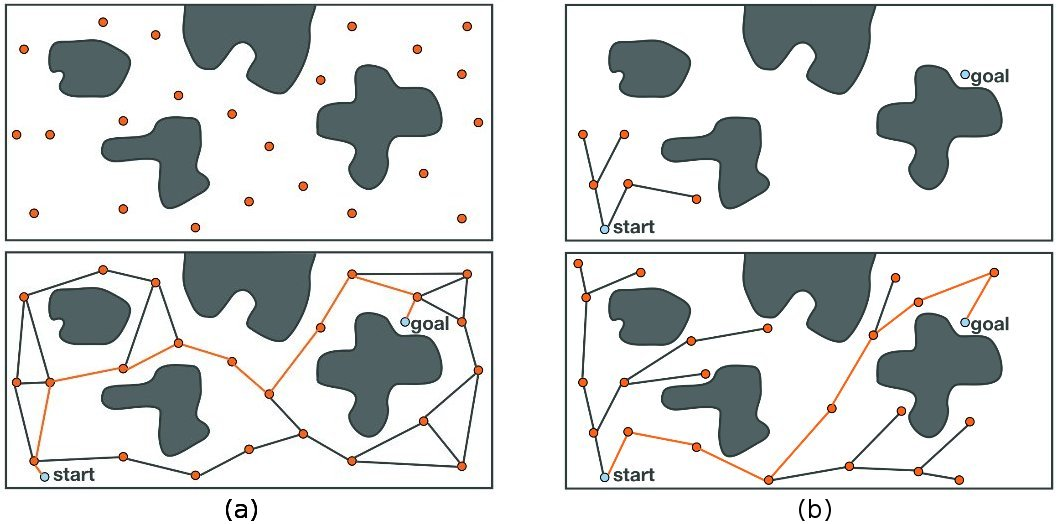
\includegraphics[width=1.0\textwidth]{images/sampling_based.jpg}
	\caption[Sampling based algorithms]{Probabilistic roadmap (left) and tree based approach (right)}
	{\scriptsize Image source: \citep{omplPrimer}
	\label{fig:sampling_based}
\end{figure}

Generally can be said that the tree based approaches are more adequate for \emph{single query planning} because the tree usually does not has to cover the whole free state space. A roadmap could be reused for subsequent queries. As the most methods also require the search of a nearest neighbour, the utilized distance metric is also a crucial part within sampling-based motion planning as it is not always easy to identify the optimal method for finding nearby states in systems with large degrees of freedom.  

\section{The MoveIt! motion planning framework}

MoveIt\footnote{http://moveit.ros.org} is an open source framework for motion planning. It is the successor of the previous arm navigation stack and therefore fully integrated into ROS. MoveIt was originally developed by Willowgarage\footnote{http://www.willowgarage.com} but since April 2012 it is maintained by the Open Source Robotics Foundation (OSRF). Figure\ref{fig:moveit_arch} gives an overview about the system architecture. Central part of the framework is the \texttt{move\_group} node which  provides a rich set of ROS topics and services that can be used to solve planning problems and execute calculated motion plans on connected hardware. Configuration of that node happens via the parameter server. It requires a complete kinematic and semantic description of the robot setup and a lot of other configuration parameters which will be described in subsequent sections. Various important parts of MoveIt are implemented as plugins. The default inverse kinematics plugin uses the Kinematics and Dynamics Library\footnote{http://www.orocos.org/kdl} (KDL) for solving IK problems. The utilized planning plugin uses the Open Motion Planning Library\footnote{http://ompl.kavrakilab.org} (OMPL), which is a framework that contains implementations of many different sampling based motion planning algorithms. Therefore it is possible to choose, which one of those algorithms to use during planning requests. \\

\begin{figure}[ht]
	\centering
  	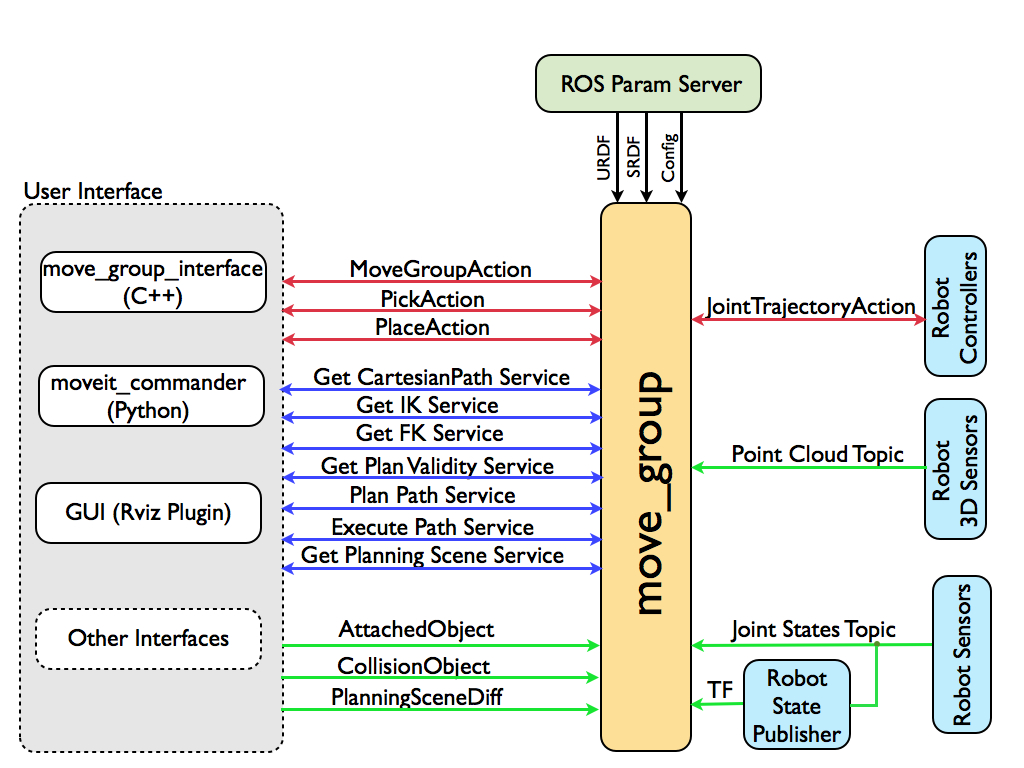
\includegraphics[width=0.75\textwidth]{images/moveit_architecture.jpg}
	\caption[Moveit architecture]{MoveIt architecture}
	{\scriptsize Image source: \url{http://moveit.ros.org/documentation/concepts}}
	\label{fig:moveit_arch}
\end{figure}

MoveIt maintains a planning scene which is an internal representation of the world, including the robot and it's environment. The base is a description of the robot and it's various planning groups. 
The kinematic description needs to be available in form of a URDF model. Necessary steps to create that model are described in Section\ref{sec:urdf}. Based on that URDF model, a semantic description (SRDF) is created that contains additional information about the setup, as explained in Section\ref{sec:moveit_assistant}. On top of those static descriptions, MoveIt allows to modify the planning scene on runtime via appropriate ROS topics.\\

To keep track of the current state of the robot MoveIt needs to be informed continuously about actual joint states. This is done via publishing the joint states to a specific topic. If there are additional objects within the robot's workspace they also have to be added to the planning scene. This can be done either by explicitly adding them via the corresponding topic or by integrating sensor information like Kinect camera data. MoveIt can then take those objects into account during motion planning and avoid collisions. But some collisions are intended. For example if an object has to be picked up, the gripper has to get in contact to this object. That means, collision checking for specific objects has to be (temporary) disabled to allow those controlled collisions. Therefore MoveIt maintains an \emph{AllowedCollisionMatrix} to which objects can be added or removed. The connection to the hardware happens via the \emph{FollowJointTrajectory} action interface. Each robot component has to provide this interface if it is intended to be control via MoveIt. This interface consists of a set of ROS topics that provide trajectory execution functionality and also allow monitoring the current execution status. The implementation and usage of a ROS node that provides the necessary interface is described in section \ref{sec:hardware_adapter}.

\section{Creating the URDF model of the robot setup}
\label{sec:urdf}

The \emph{Unified Robot Description Format} (URDF) is a markup language, designed to describe robots. The description happens in text files, in a special XML format. The most important elements in the XML specification\footnote{http://wiki.ros.org/urdf/XML} are:

\begin{itemize}

\item \textbf{<link>} \\
Describes the all necessary properties of a specific robot link. Each link must have a unique name. The visual, inertial and collision details are configured in the corresponding subtags of the link element. The visual part as well as the collision model can either be composed from primitive shapes
or from mesh files. If mesh files are used it is important that they are not to complex. Especially for the collision model it is recommended to use a simplified model to avoid a performance loss.

\item \textbf{<joint>} \\
Describes the properties of a joint. A joint is a connection between two links, having exactly one parent and one child link. Each joint states a new reference frame for it's child link and it is positioned relative to it's parent frame. A \emph{fixed} joint is a rigid connection between parent and child link. There are different types of joints available but for the current project only \emph{revolute} joints\footnote{Rotational joint with one degree of freedom} are of interest. Details like limits, axis orientation and dynamic properties can be configured in the corresponding subtags of the joint element.

\end{itemize}
\begin{figure}[ht]
	\centering
  	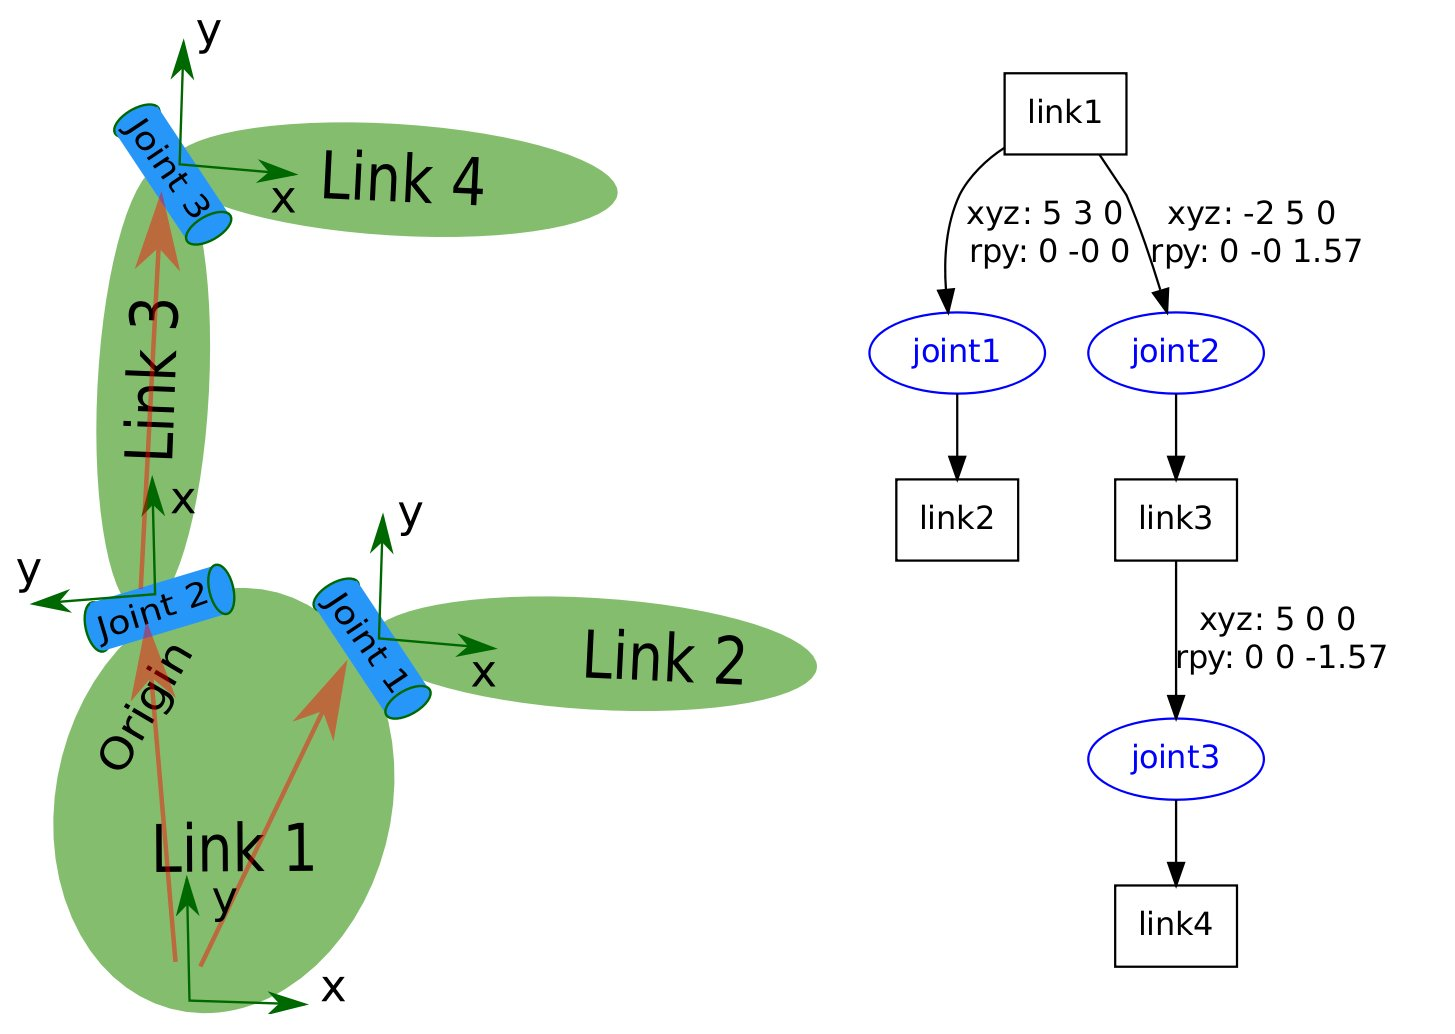
\includegraphics[width=0.75\textwidth]{images/urdf_chain.jpg}
	\caption[URDF graph]{URDF graph}
	{\scriptsize Image source: http://wiki.ros.org/urdf/Tutorials/Create your own urdf file}
	\label{fig:urdf_graph}
\end{figure}
Those elements are used to form the URDF graph that exactly describes the kinematic chain of the robot components and their placement relative to each other as visualized in Figure\ref{fig:urdf_graph}. This description can get very large as a lot of different components are involved. So it is possible to organize it into a set of text files, each one describing one part of the whole. For example one file describes the arm itself. Other files can then use that description and insert multiple instances of that arm. The \texttt{xacro} ROS package provides the necessary functionality to combine all those text files into one XML string. \emph{XACRO} stands for \emph{XML Macro} and is designed to parse xacro files and combine them into one single XML document, containing the resulting URDF description.\\

The URDF description of the IIS robot setup is spread across multiple packages, located in the \texttt{iis\_hardware} stack. Arm and gripper descriptions are located in seperate packages (\texttt{lwr\_description} and \texttt{schunk\_description}), the \texttt{iis\_robot} package brings all the components together. The modelling process started with the search for pre-existing URDF descriptions of the required robot components. A suitable description of the Schunk SDH gripper was taken from the \texttt{schunk\_description} ROS package. A model of the KUKA LWR arm was found in the Github repository\footnote{https://github.com/RCPRG-ros-pkg/lwr\_robot/tree/hydro-devel/lwr\_defs} of the \emph{Robot Control and Pattern Recognition Group}\footnote{University of Warsaw (http://robotyka.ia.pw.edu.pl/twiki/bin/view/Main)}. The other parts of the model, namely the robot torso and the table had to be created. The descriptions are located in a seperate files within the \texttt{uibk\_robot} package (\texttt{torso.xacro} and \texttt{table.xacro}).

The mesh files, used in the description of the robot torso have been exported from the V-Rep simulation scene. For the visual part, the mesh was taken as it is. For the collision model, the width of the original mesh was increased to provide some safety padding. Moreover a cylinder with a diameter of 40cm was added in the head area to ensure that the planner avoids accidental hits in this sensitive region. Figure\ref{fig:torso_col} shows the visual and the collidable part of the torso model.
\begin{figure}
	\centering
  	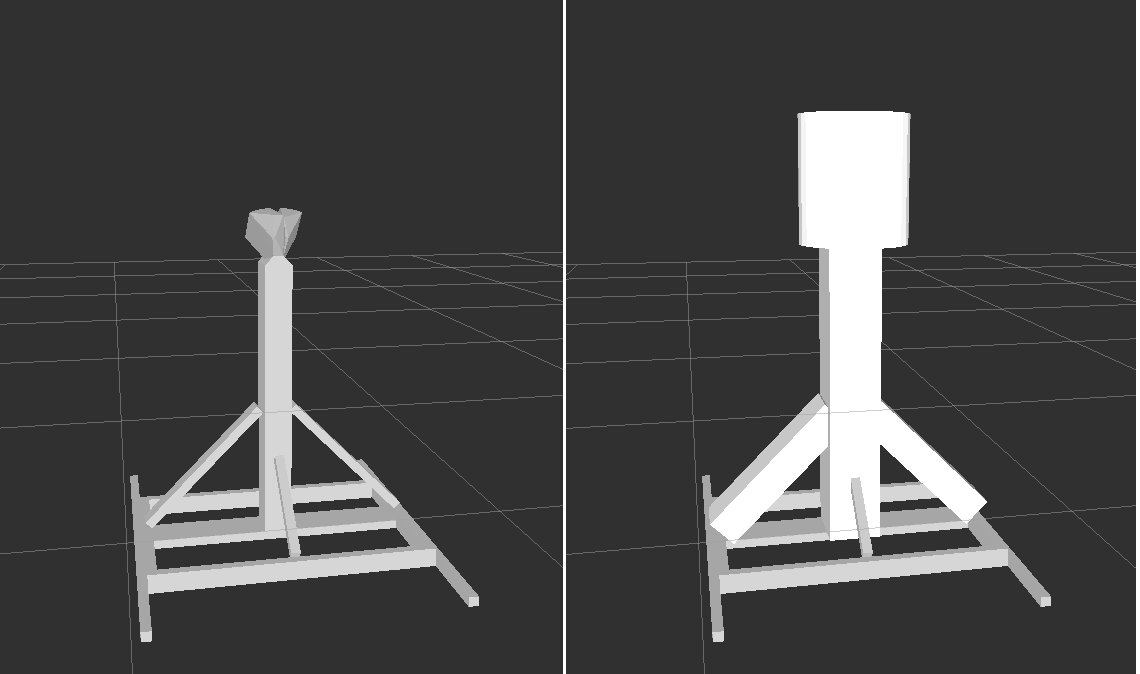
\includegraphics[width=1.0\textwidth]{images/torso.jpg}
	\caption[Visual and collidable model of torso]{Left image shows visual part, right image the collidable part of the torso}
	\label{fig:torso_col}
\end{figure}
The table was modelled from primitive shapes. It was taken care that the size of the table can easily be adjusted, as can bee seen in Listing\ref{lst:table}. The collision model of the table is also slightly larger than the visual part to provide some safety margins.
\lstset{language=XML,style=customxml}
\begin{minipage}{\linewidth}
\begin{lstlisting}[caption={XML snippet, inserting the table model into the URDF}, label=lst:table]
<!-- draw the table relative to the origin -->
<xacro:model_table name="table" 
	     parent="world"
	     length="2.22"
	     width="0.8">
	<!-- Place the table relative to the world reference frame -->
	<origin xyz="-0.029 -0.3 0" />
    
</xacro:model_table>
\end{lstlisting}
\end{minipage}

When attaching the two grippers it showed that the offset between gripper wrist and last arm link was not correct. To correct that issue the file \texttt{sdh\_with\_connector.xacro} was created which simply places an additional ring between the last arm link and the gripper.\\

The file \texttt{iis\_robot\_table.xacro} draws all the pieces together. It describes the whole setup, consisting of the torso, two arms, two grippers and the table. The root element of the model hierarchy is a link called \texttt{world\_link}. Torso, table and both arms are positioned relative to that root link. Changing the world reference frame could easily be achieved by shifting the root link to a new position. Figure\ref{fig:robot_table} shows a visualization of the URDF description.
\begin{figure}
	\centering
  	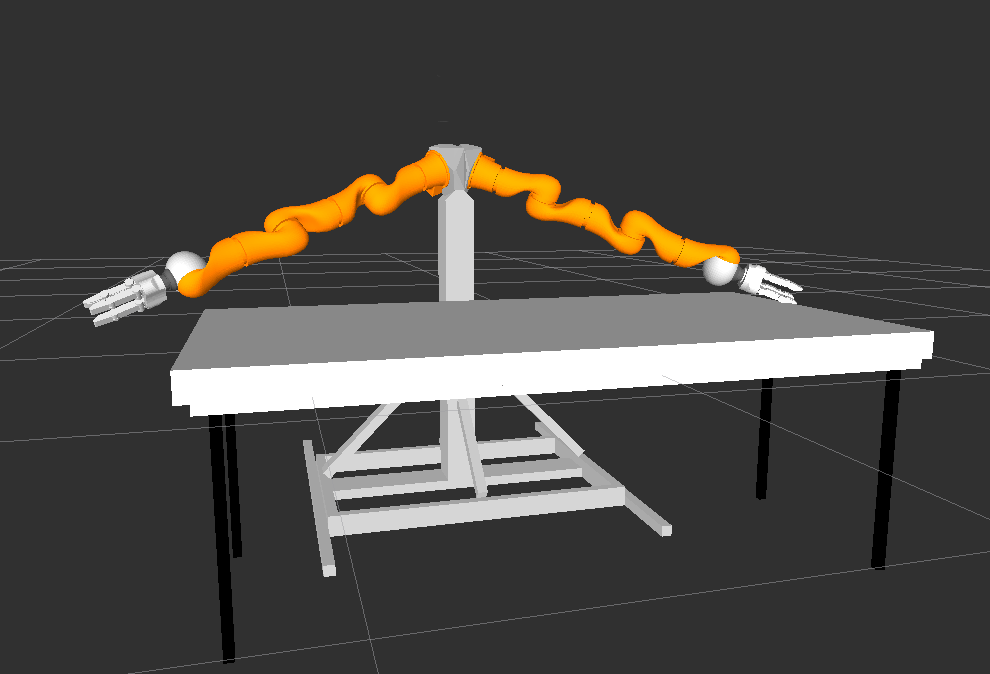
\includegraphics[width=0.75\textwidth]{images/iis_robot_table.png}
	\caption{URDF description in RViz}
	\label{fig:robot_table}
\end{figure}

\section{Configuring the planning tools}
\label{sec:moveit_assistant}

The MoveIt configuration package is created, using the \emph{MoveIt Setup Assistant}. Precondition is an existing URDF description of the robot setup which was created in the previous step.
The setup process comprised of the following steps:

\begin{itemize}

\item \textbf{Computating the self collision matrix}

The self collision matrix consists of pairs of robot links that can safely be excluded from collision checking. Neighbouring links for example are in permanent collision. Collisions between other links can never happen because they are simply too far apart. The Setup Assistant calculates a large number of different robot configurations and tracks for link pairs that are mostly always in collision and pairs that are never in collision. The self collision matrix can be adjusted manually if necessary. Excluding a large number of link pairs raises performance during motion planning because collision checking is an expensive process.

\item \textbf{Defining the planning groups}

Each planning request in MoveIt is done against one of the defined \emph{planning groups}. A planning group is a group of links and joints within the model that can be seen as one logical component. Planning groups are defined for both arms and grippers. The configuration for the arms also requires the definition of the utilized IK solvers but currently only the default KDL solver is available. An additional planning group, called \texttt{both\_arms} allows planning requests for both arms simultaneously.

\item \textbf{Defining the end effectors}

End effectors are the left and the right gripper. Each end effector has a name and consists of one of the predefined planning groups, a parent group and the parent link which is the last link in the kinematic chain of the parent group.

\item \textbf{Generate the configuration files}

After completing all the configuration steps the configuration package can be generated. Therefore a package name has to be specified which was set to \path{uibk_robot_moveit_config}. This package is a prototype, containing a large number of predefined configuration files. Some of those files have to be extended manually, adding additional information about available robot controllers and sensors. 

\end{itemize}

Completing the last step results in a ROS package, containing necessary configuration and launch files for the given robot setup. The semantic robot description can be found in the \path{iis_robot.srdf} file. It contains previously defined parameters like the self-collision matrix, planning groups and end effectors. The configuration package can be tested, running the following command on the command line:
\begin{quote}
\begin{verbatim}
roslaunch uibk_robot_moveit_config demo.launch
\end{verbatim}
\end{quote}
This commands launches a \path{move_group} node in demo mode, using the previously created configuration files and starts an instance of RViz with the motion planning plugin. There it is possible to switch between the planning groups, set start and target configurations, do planning requests and visualize the outcome. The setup can be modified by launching the Setup Assistant again, using the \path{setup_assistant.launch} file from this package.

\section{Connecting MoveIt to the existing robot control interface}
\label{sec:hardware_adapter}

Now MoveIt is configured and ready to handle planning requests for the robot setup. But execution of the resulting trajectories is still impossible because of the missing connection between MoveIt and the involved robot hardware. Each component that is intended to be controlled by MoveIt needs to provide the \emph{FollowJointTrajectory} action interface, as defined in the \texttt{control\_msgs} package. This is a special kind of ROS interface that allows to send trajectories to robot components and monitor the execution status. As the existing control interface of the IIS robot components does not fulfil these requirements, an additional node is necessary that is capable of executing trajectories, using the existing infrastructure.\\

The planning outcome of MoveIt is a time parametrized trajectory, expressed by the \emph{JointTrajectory} message type. This message consists of a set of waypoints. A waypoint is a joint configuration, described by the tuple $(p,v,a,t)$ where $p \in \mathbb{R}^n$ are the positions, $v \in \mathbb{R}^n$ the velocities and $a \in \mathbb{R}^n$ the accelerations at time $t$ and $n$ is the number of involved joints. Those waypoints mark the important points along the path, the manipulator has to move. The controller needs to be able to translate this trajectory into a sequence of suitable motor commands. Just sending the joint positions within the waypoints to the robot would not suffice as a trajectory is also constrained in terms of \emph{velocities} and \emph{accelerations} over \emph{time}. Therefore the controller needs to be able to interpolate between the subsequent waypoints and calculate intermediate joint positions based on the loop rate of the control cycle. This interpolation is a difficult task and the implementation would be beyond the scope of this project. But the required functionality is already available within the \path{ros_control} stack\footnote{http://wiki.ros.org/ros\_control}. Those packages are created to integrate and control robot hardware in a generalized way, facilitating the usage of existing controllers on different robots. 

\subsection{ROS control stack overview}

\begin{figure}
	\centering
  	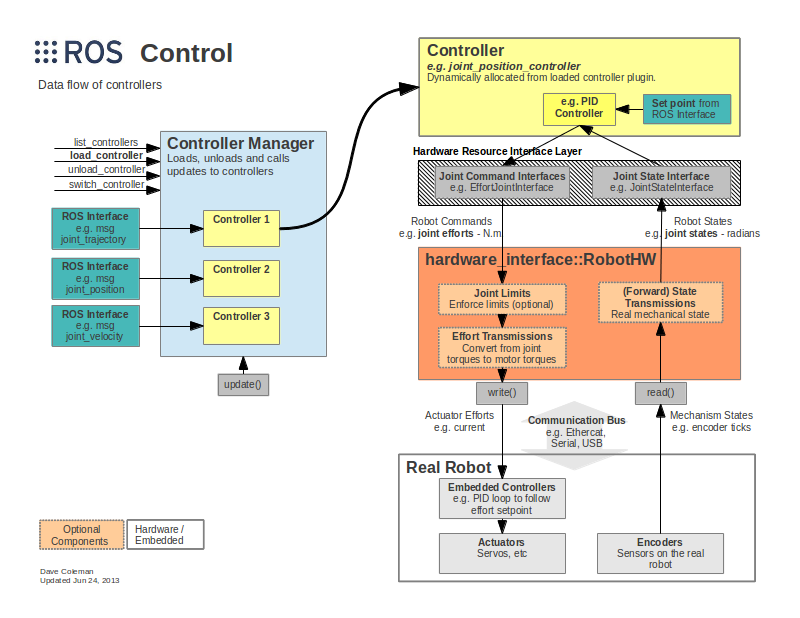
\includegraphics[width=1.0\textwidth]{images/ros_control.png}
	\caption{ROS control architecture}
	{\scriptsize Image source: http://wiki.ros.org/ros\_control}
	\label{fig:ros_control}
\end{figure}
Figure\ref{fig:ros_control} shows an architectural overview of the ROS control stack. The required infrastructure for using generic controllers is mainly provided by two components:

\begin{itemize}

\item \textbf{RobotHW} \\

This is the abstract base class for robot hardware abstraction. It's main purpose is to send commands to the hardware and retrieve state data. The \emph{RobotHW} also maintains a set of \emph{hardware ressource interfaces}. Each generic controller needs a special kind of interface for controlling joints or read their current state. Concrete implementations have to register the required interfaces. For retrieving state data, a \emph{JointStateInterface} is required. Controllers using that interface can query it for a specific joint and ask for the current state. Sending commands to the joints is done via subtypes of the of the abstract \emph{JointCommandInterface}. The \emph{PositionJointInterface} for example allows to send target positions to registered joints. Other implementations are \emph{JointEffortInterface} and \emph{JointVelocityInterface}. Which interfaces are provided depends on the way how the actual hardware is controlled.

\item \textbf{ControllerManager} \\

The \emph{ControllerManager} is responsible to maintain a set of controllers. It provides a ROS interface that allows to load, start and unload controllers and for switching between them. During the control cycle, the \emph{RobotHW} is forced to read current state from the hardware. Then the \emph{ControllerManager} is triggered to update the active controllers based on the current time step. The commanded values are then sent back to the concrete hardware. This control cycle is intended to run in real time when interacting directly with the hardware. Controllers are usually configured on the parameter server and loaded on demand, using the ROS interface of the \emph{ControllerManager}. Custom controllers can be created by inheriting from the abstract  \emph{ControllerBase} class.  

\end{itemize}

\subsection{Designing the hardware adapter}

The \emph{hardware adapter} is an independent ROS node that acts as connection between MoveIt and the simulated or real hardware. It provides the necessary infrastructure for using generic controllers from the \texttt{ros\_control} packages. Figure\ref{fig:hardware_adapter} gives an overview about the hardware adapter architecture. The \emph{UibkRobotHW} is a subclass of \emph{RobotHW} and represents the connection to the robot. It maintains the complete state of all joints in the connected components. Joints are represented by the \emph{Joint} datatype, consisting of a unique joint name, state parameters and a commanded target position. For controllers, the \emph{UibkRobotHW} class provides a \emph{JointStatesInterface} and a \emph{JointPositionInterface}. Active controllers use those interfaces to access the current state and for commanding target positions. 

The \emph{UibkRobotHW} utilizes a set of \emph{JointStateAdapters}, each one representing a connection to one specific robot component. During the control cycle the \emph{JointStateAdapters} read current joint states from the appropriate topics and send commanded values back to the hardware.
\begin{figure}[h]
	\centering
  	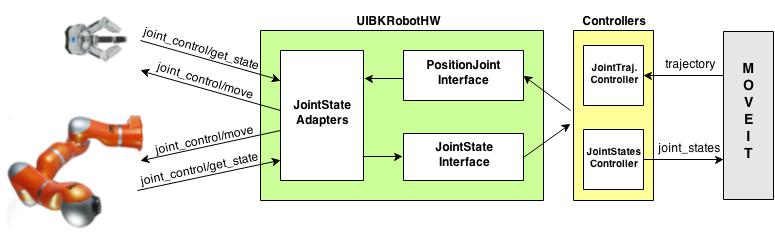
\includegraphics[width=1.0\textwidth]{images/hardware_adapter.jpg}
	\caption{Hardware adapter architecture}
	\label{fig:hardware_adapter}
\end{figure}
The \emph{JointStateAdapters} are created during initialization, based on the configuration settings. After creation, each \emph{JointStateAdapter} waits a certain amount of time for an initial joint states message. If it does not receive such a message before timeout, it will automatically shut down for safety reasons and report an error. This is very important as the \emph{JointStateAdapter} imediately begins to send joint positions after initialization. The position to be sent is initially the currently known position, as long as no other values have been commanded by the controllers. Therefore the initial position always has to be known, otherwise dangerous and rapid robot motions could occur on startup. The adapter configuration happens via the parameter server. Available configuration parameters are:

\begin{itemize}

\item \textbf{\texttt{adapter\_list}} \

Contains a list of all \emph{JointStatesAdapters} that have to be created. For each adapter name mentioned in this list a detailed configuration is required. The subsequent parameters have to be configured for each single adapter.

\item \textbf{\texttt{joint\_state\_topic}} \

The name of the topic where a specific adapter listens for joint states. The expected message type  \texttt{sensor\_msgs/JointStates}. This parameter is mandatory.

\item \textbf{\texttt{readonly}} \

This parameter is optional. If true then the adapter will only listen for joint states but not publish commanded values.

\item \textbf{\texttt{joint\_command\_topic}} \

The name of the topic the adapter should use to publish the commanded values to. The expected message type is \texttt{std\_msgs/Float64MultiArray}. This parameter is mandatory if the adapter is not configured to be read only.

\item \textbf{\texttt{joints}} \

A list of joint names that should be controlled by the adapter. The order in this list also determines the order of the values in the published message.

\item \textbf{\texttt{joint\_name\_prefix}} \

This parameter can be used to be able to uniquely identify joints. For example both arms are using the same joint names (\texttt{arm\_0\_joint}, \texttt{arm\_1\_joint},\ldots). But in a URDF model,  joint names have to be globally unique. Therefore the prefix can be used to prepend the original name to achieve uniqueness. A value of \texttt{right\_} for example will lead to the joint names \texttt{right\_arm\_0\_joint}, \texttt{right\_arm\_1\_joint},\ldots).

\end{itemize}

An example configuration can be found in Listing\ref{lst:adapter_config}. As the topic names, used by the \emph{JointStateAdapters} can be configured freely, the hardware adapter is able to interact with the simulator and the real robot as well, as both of them provide exactly the same ROS interface.

\begin{minipage}{\linewidth}
\lstinputlisting[caption={Adapter configuration for left arm and gripper}, label=lst:adapter_config]{code/adapter_config.yaml}
\end{minipage} \\

During hardware adapter startup an instance of the \emph{UibkRobotHW} and \emph{ControllerManager} is created from configuration. As the control loop must not be interrupted by ROS callback functions, it is launched in a separate thread after completing initialization, using a loop rate of 100hz. On each iteration the exact time since the last step is calculated. The \emph{ControllerManager} then updates all registered controllers based on current state and time since last iteration. After handling the controllers, the \emph{JointStatesAdapters} are forced to send the commanded values to the hardware. The ROS callback functions are handled in the original thread.\\

After starting the hardware adapter, the required controllers have to be loaded and started. This is usually done, by using the corresponding ROS services, provided by a running \emph{ControllerManager} instance, but the \texttt{controller\_manager} package contains a tool named \texttt{spawner} that simplifies the starting process. The configuration of each controller has to reside on the parameter server. Utilized controllers are the \emph{JointTrajectoryController} and the \emph{JointStateController}. The \emph{JointTrajectoryController} provides the required \emph{FollowJointTrajectory} action interface for a group of joints. For each robot component a separate \emph{JointTrajectoryController} is used. The \emph{JointStateController} publishes the collected states of all robot joints at once to the \texttt{joint\_states} topic, which is used by MoveIt to monitor the robot configuration.

\subsection{Launching the hardware adapter}
\label{sec:launch_moveit}

The file \texttt{hardware\_adapter.launch}, located in the \texttt{uibk\_moveit\_adapter} package was created to handle the necessary configuration parameter upload and launch the hardware adapter node for the simulator and the real robot as well. As can be seen in Listing\ref{lst:adapter_config}, the configured topic names for the \emph{JointStateAdapters} are defined, using \emph{relative} graph resource names (i.e. without trailing slash). The required instance is than accessed by simply shifting the node into \texttt{simulation} or \texttt{real} namespace. This is realized, specifying the \texttt{config\_name} parameter of the launch file. The command line statement
\begin{verbatim}
roslaunch uibk_moveit_adapter hardware_adapter.launch config_name:=simulation
\end{verbatim}
launches the hardware adapter in \texttt{simulation} namespace.\\

After launching the hardware adapter node, the required controllers are loaded and started. The node provides feedback information about the state and errors during startup process on the console output. It is crucial that the joint state topics of simulator or real robot are available before launching the hardware adapter node, otherwise it will not be able to work because of missing initial joint states. After successful startup, the additional controller topics can be found in the corresponding namespace.

\section{Adjusting the MoveIt configuration}

The prerequisites are now made for connecting MoveIt to the (simulated or real) robot. The last remaining step is to adjust the MoveIt configuration for establishing a connection to the \emph{FollowJointTrajectory} controllers. Therefore the configuration file \path{controllers.yaml} was created in the \path{uibk_robot_moveit_config} package. It contains a list, describing the available controllers. Each controller description contains the name of the controller, it's action namespace, the controller type and a list, containing the names of the controlled joints.\\

For starting MoveIt, the launch file \path{moveit_planning_execution.launch} was created. This file is intended to launch a \texttt{move\_group} node either for simulated or real robot, together with the corresponding hardware adapter. The namespace can be selected using a boolean parameter named \texttt{simulation}. The statement
{\small 
\begin{verbatim}
roslaunch uibk_robot_moveit_config moveit_planning_execution.launch simulation:=false
\end{verbatim}}
launches a MoveIt configuration, connecting the \texttt{move\_group} instance to the real robot. The launch file also starts RViz configured with the motion planning plugin. This is used for visualizing the planned trajectories and can also be used to test the connection to the robot by making planning requests and execute the resulting trajectories.